The goal of PIP is to evaluate queries on variables sampled from both discrete and continuous distributions as well as to provide tools to aid in the statistical analysis of those results.  Uncertainty in PIP is represented via random variables.  When instantiating a random variable, users specify both a distribution for the variable to be sampled from, and a parameter set for that distribution.  A single variable may appear simultaneously at multiple points within the database, so PIP assigns each variable a unique identifier that allows sampling processes to generate consistent values for the variable.

In addition to representing uncertainty in values for individual cells in a table, PIP represents per-tuple uncertainty with c-tables.  Each tuple is tagged with a condition that must hold for the variable to be present in the table.  C-table conditions are expressed as a boolean equation of \textit{atoms}, arbitrary inequalities of random variables.  The independent probability, or \textit{confidence} of the tuple is the probability of the condition being satisfied.  

\subsection{Random Variables}
Every random variable is created from by specifying a distribution and a set of parameters for that distribution.  For example, we write $[X=>Normal(\mu,\sigma^2)]$ to represent a random variable named X that follows a Normal distribution with a mean of $\mu$ and a standard deviation of $\sigma^2$.  In this way, PIP is agnostic to the distribution which a variable is sampled from; arbitrary problem-specific distributions may be created and seamlessly integrated into PIP's infrastructure.  

When defining a distribution, programmers need only include a mechanism for sampling from that distribution.  However, if it is possible to efficiently compute or estimate the distribution's probability density function ($PDF$), cumulative distribution function ($CDF$), or inverse cumulative distribution function ($CDF^{-1}$), these may be included to increase PIP's efficiency.  The process of defining a variable distribution is described further in Section \ref{sec:implementation}.  

Though PIP abstracts the details of a variable's distribution from query evaluation, it distinguishes between discrete and continuous distributions.  As described in Section \ref{sec:background}, existing research into c-tables has demonstrated efficient ways of querying variables sampled from discrete distributions.  PIP employs similar techniques when it is possible to do so.

Multiple continuous random variables may be combined algebraically into a random variable expression.  Random variable expressions may be used to define joint distributions, to build more complex distributions, or may be created as a side effect of query evaluation.  Though random variable expressions are interchangeable with regular random variables in general, there are several instances where they receive special treatment.  In particular, it is necessary to ensure that within a given sample all instances of a given random variable assume the same value; the expectation of a random variable expression is obtained based on a consistent set of samples for all of its component random variables.

Finally, constraint atoms are conditional formulas of random variables.  Such formulas may be equalities if all variables in the fomula are discrete, otherwise they must be an inequality; the probability of a continuous variable adopting an exact value is zero.  Given a constraint atom $C$, its probability $P[C]$ is the probability of selecting variable assignments that satisfy the formula.  Constraint atoms are used to express a tuple's condition.  By adding constraint atom columns to a table, a tuple's presence in the table becomes dependent on the constraint atom being true; the tuple's presence is based on the conjunction of all its component atoms.

\subsection{Variable Definition}
Before evaluating a query on random variables, the variables must first be defined.  This process takes one of two forms.  PIP uses a repair-key operator similar to that used in \cite{KochMayBMS2008} to define discrete distributions.  Conceptually, this operator identifies tuples that share key values, and ensures that only one of the two tuples is present in the database at any given moment.  

Continuous variables may be created inline with the create-variable operation.  This function takes a distribution class and parameters, and outputs a new variable.  For example, the following query outputs a variable delivery time for a given order.

\begin{verbatim}
select orders.order_id, orders.item_id,
       CREATE_VARIABLE (`Normal', params.mean,
         params.std_dev) AS delivery_time
from   orders, params
where  orders.item_id = params.item_id;
\end{verbatim}

\subsection{Query Processing}
Query evaluation proceeds in two phases: Query and Sampling.  During the query phase, PIP evaluates a query rewritten to employ the c-tables relational algebra extensions described in Section \ref{sec:background}.  Selection clauses not involving random variables are handled traditionally, while those involving one or more random variables instead tag the output tuple with an equivalent condition clause.  For example, the query:

\begin{verbatim}
select *
from   input_table
where  fixed_column = 3
 and   4 > variable_column;
\end{verbatim}
%
is rewritten to
%
\begin{verbatim}
select *, constraint(`4 > variable_column')
from   input_table
where  fixed_column = 3;
\end{verbatim}

Queries are also modified to ensure that these newly created constraint columns interact with projections properly.  All select statements are modified to automatically output all constraint columns in their input tables and subqueries.  The only exception to this rule is in the case of sampling selection.  Behaving similarly to aggregate selects, a sampling select projects away uncertainty by including a sampling operator such as expect(), or conf().  Note that aggregate and sampling selects are not mutually exclusive.  Indeed, due to exponential complexity of losslessly representing arbitrary aggregate output conditions (An aggregate can generate $2^{N}$ distinct outputs in the number of input rows), PIP requires that aggregate selects perform sampling. 

\subsection{Per-Row Sampling}
Given a target expression (that may contain random values) as well as a set of constraints, the sampler computes the expression's expectation by first subdividing the problem as described in Section \ref{subsec:independence}.  These groups are subsequently divided into two categories: Groups containing at least one variable contained in the target expression are marked for sampling.  The volume of the probability space defined by all constraints must be computed, but storage overheads may be avoided for those groups not directly relevant to the target expression; these groups are marked for integration.  Additionally, if the group contains only one variable, the value may be computed exactly using the variable's CDF if one is available.

The remaining groups are sampled to obtain values for Monte-Carlo estimation of the target expression's expectation.  By default, these samples are obtained through naive rejection sampling.  Variables are selected from the distribution $\frac{\chi(\vec{x})p(\vec{x})}{\int_{\vec{a}} \chi(\vec{a})p(\vec{a})}$ by sampling according to $p(\vec{x})$ and discarding values that do not satisfy $\phi(\vec{x})$.  This distribution is normalized according to the frequency with which samples are discarded.  

If any of the variables have a CDF available, PIP first attempts to obtain weak bounds on the variable as described in Section \ref{subsec:icdf}.  If such bounds are available, PIP can use the variable's CDF and inverse CDF to restrict its sampling to within the weak bounds.  If the weak bounds are actually tight bounds, no samples will be discarded.  However, even if some samples are rejected, the bounds reduce the drop frequency.  When computing the volume of the probability space defined by the constraints, the values are re-normalized according to the fraction of the CDF located within the bounds.

A final option available to PIP is the Metropolis algorithm.  Metropolis has a high initialization cost: Prior to sampling, at least one value $\vec x$ satisfying $\theta(\vec x)$ must be found (though it need not be selected according to any specific probability distribution), and a significant number of burn-in iterations must be run and discarded.  Furthermore, every sampling step requires many metropolis iterations to achieve sufficiently independent samples.  However, Metropolis is guaranteed to stay within the constraint bounds and no samples will be rejected.  Thus, we can estimate the work required for both Metropolis and Naive rejection sampling.

$$W_{metropolis} = C_{burn\ in} + [\#\ samples] \cdot C_{steps\ per\ sample}$$
$$W_{naive} = \frac{1}{1-P[reject]} \cdot [\#\ samples]$$

By generating a small number of samples for the subgroup, PIP generates a rough estimate of $P[reject]$.  If this value is lower than $\frac{1}{\frac{C_{burn\ in}}{[\#\ samples]} + C_{steps\ per\ sample}}$, Metropolis sampling is used instead of rejection sampling.  Note that if CDFs are available for one or more component variables, PIP uses the probability of rejecting samples chosen from within the weak bounds.

The single-row sampling process is sumarized in Figure \ref{fig:roadmap}

\begin{figure}
\begin{center}
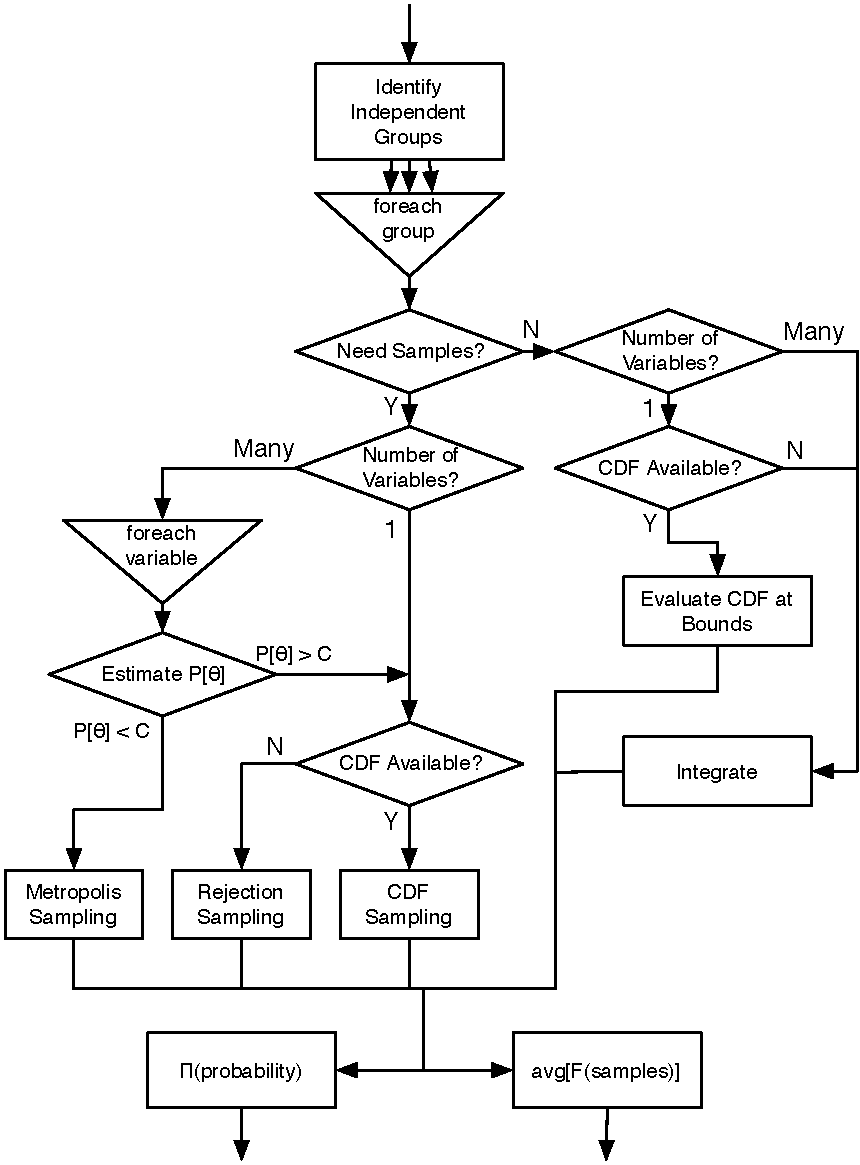
\includegraphics[width=3in]{graphics/roadmap.pdf}
\caption{\textbf{The PIP Single-Row sampling process}}
\label{fig:roadmap}
\end{center}
\end{figure}

\subsection{Aggregate Sampling}
The complexity introduced by aggregate operations, coupled with the frequency with which they appear at the root of a query plan, makes them an ideal point at which to perform sampling.  We begin with the simplest form of aggregate expectation, that of an aggregate that obeys linearity of expectation ($\left<f(\vec{x})\right> = f(\vec{\left<x\right>})$), such as sum().  

Such aggregates are straightforward to implement: per-row expectations of $f(\vec x)\chi(\vec x)$ are computed, and aggregated (e.g., summed up).  Of note however, is the effect that the operator has on the variance of the result.  In the case of sum(), each expectation can be viewed as a Normally distributed random variable with a shared, predetermined variance.  By the law of large numbers, the sum of a set of $N$ random variables with equal variance $\sigma$ has a variance of $\frac{\sigma}{\sqrt{N}}$.  In other words, when computing the expected sum of $N$ variables, we can reduce the number of samples taken for each individual element by a factor of $\frac{1}{\sqrt{N}}$.

If the operator does not obey linearity of expectation (e.g., computing the maximum), either the aggregate must be designed with expectation computation in mind, or the aggregate must be run on a set of sampled worlds in parallel.  This latter technique is a worst-case approach to the problem; it may be necessary to re-run the aggregate if an insufficient number of sample worlds are generated. Note however, that this is still more efficient than re-running the entire query.

The max() aggregate can be implemented more efficiently, particularly when the target expression is a constant (ie, a value that is certain for the row in question).  Given a table table sorted over descending values of the target expression, PIP estimates the probability that the first element in the table (the highest value) is present.  The aggregate expectation is initialized as the product of this probability and the first element.  The second term is maximal only if the first term is not present; when computing the probability of the second term, we must compute the probability of all the second term's constraint atoms being fulfilled while at least one of the first atom's terms is not fulfilled.  Though the complexity of this process is exponential in the number of rows, the probability of each successive row being maximal drops exponentially.  

